\documentclass[12pt,a4paper]{article}
\usepackage[english]{babel}
\usepackage[utf8]{inputenc}
\usepackage{fancyhdr}
\usepackage{hyperref}


% Math
\usepackage{bm}

% graphics
\usepackage{graphicx}
\graphicspath{ {images/} }
\usepackage{tikz}

% date
\usepackage{datetime}
\newdateformat{specialdate}{\THEYEAR-\twodigit{\THEMONTH}-\twodigit{\THEDAY}}
\date{\specialdate\today}
\usepackage{xcolor}

% Colors
\definecolor{command}{rgb}{0.325, 1, 1}
\definecolor{flag}{rgb}{1, 0.325, 0.325}
\definecolor{param}{rgb}{0.825, 0.825, 0.825}

%renew commands
\renewcommand{\contentsname}{Tabla de contenidos}

\begin{document}
	\begin{titlepage}
		\centering
		
\includegraphics[width=0.4\textwidth]{logo-ugr.png}\\*
		{\scshape\LARGE Universidad de Granada \par}
		{\large \date{\specialdate\today}\par}
		\vspace{1cm}
		{\LARGE\bfseries Zabbix\par}
		\vspace{1.5cm}
		{\scshape\large Ingeniería de Servidores\par}
		\vspace{2cm}
		{\Large\itshape Lukas Häring García 3ºC\par}
	\end{titlepage}
	
	\tableofcontents
	
	\newpage
	
	\section{Zabbix}
	\textbf{Zabbix} es un sistema de monitorización de redes creado por Alexei Vladishev. Está diseñado para monitorizar y registrar el estado de varios servicios de red, Servidores y hardware de red[1].
	\newline
	\newline
	Esta práctica se centrará en la monitorización de servidores, en nuestro caso, virtuales. Por lo que vamos a utilizar los dos sistemas operativos que hemos estado utilizando en prácticas anteriores, Ubuntu[2] y CentOs[3].
	\newline
	\newline
	\textbf{Zabbix} se puede instalar como \textit{servidor} únicamente en \textbf{Ubuntu}, por lo que será nuestro servidor, uno de nuestros \textit{agentes} (monitorizado) y nuestro \textit{frontend}. Utilizaremos \textbf{CentOS} únicamente para monitorizarlo.
	
	\subsection{Instalación Zabbix}
	
		Suponiendo que hemos completado las prácticas anteriores correctamente y estamos en modo \textbf{super-usuario} o \textbf{kernel}.
		
		\subsubsection{Intalación Zabbix en Ubuntu}
		 Supondremos además que tenemos \textbf{wget} y \textbf{apt} instalado
		\newline
		\newline
		
\begin{tikzpicture}[node distance=-0.5em]
			\node[
				anchor=north,
				draw=black,
				fill=black,
				inner xsep=0.5cm,
				inner ysep=0.2cm,
				line width=4pt,
				text width=\textwidth - 1cm,
				align=left
			] (box) { {\color{command}\textbf{wget}} {\color{param} https://repo.zabbix.com/zabbix/3.4/ubuntu/pool/main/z/zabbix-release/zabbix-release\_3.4-1+xenial\_all.deb }};
			\node[
				fill=black,
				rounded corners
			] at (box.west) {\color{white}$\boldsymbol{>}$};
		\end{tikzpicture}
		\newline
		\newline
		Instalamos el paquete que nos hemos descargado, para ello, vamos a utilizar el commando \textbf{dpkg} que viene con el paquete \textbf{apt}
		\newline
		\newline
		
\begin{tikzpicture}[node distance=-0.5em]
			\node[
				anchor=north,
				draw=black,
				fill=black,
				inner xsep=0.5cm,
				inner ysep=0.2cm,
				line width=4pt,
				text width=\textwidth - 1cm,
				align=left
			] (box) { {\color{command}\textbf{dpkg}} {\color{param}{\color{flag} -i} zabbix-release\_3.4-1+xenial\_all.deb }};
			\node[
				fill=black,
				rounded corners
			] at (box.west) {\color{white}$\boldsymbol{>}$};
		\end{tikzpicture}
		\newline
		\newline
		Vamos a comenzar con la instalación del servidor y el \textit{frontend}. {\small (\textbf{Nota}: Cabe destacar que Zabbix hace uso de la pila \textit{LAMP}[4] para almacenar las estadísticas recogidas)} \textbf{zabbix-server-mysql} se trata de un paquete que incluye el servidor de \textbf{Zabbix} y soporte \textbf{MySQL}; \textbf{zabbix-frontend-php} es un paquete que ofrece una interfaz web escrita en \textbf{PHP}.
		\newline
		\newline
		
\begin{tikzpicture}[node distance=-0.5em]
		\node[
			anchor=north,
			draw=black,
			fill=black,
			inner xsep=0.5cm,
			inner ysep=0.2cm,
			line width=4pt,
			text width=\textwidth - 1cm,
			align=left
		] (box) { {\color{command}\textbf{apt}} {\color{param}{\color{flag} install -y} zabbix-server-mysql zabbix-frontend-php }};
		\node[
			fill=black,
			rounded corners
		] at (box.west) {\color{white}$\boldsymbol{>}$};
		\end{tikzpicture}
		\newpage
		Una vez instalado el servidor y la \textit{frontend}, vamos a configurar nuestra base de datos con el usuario predeterminado "\textit{root}".
		\newline
		\newline
		
\begin{tikzpicture}[node distance=-0.5em]
		\node[
			anchor=north,
			draw=black,
			fill=black,
			inner xsep=0.5cm,
			inner ysep=0.2cm,
			line width=4pt,
			text width=\textwidth - 1cm,
			align=left
		] (box) { {\color{command}\textbf{mysql}} {\color{param}{\color{flag}  -u} root \color{param}{\color{flag}  -p}}};
		\node[
			fill=black,
			rounded corners
		] at (box.west) {\color{white}$\boldsymbol{>}$};
		\end{tikzpicture}
		\newline
		\newline
		Vamos a crear la base de datos zabbix y configurar un usuario, todo esto utilizando el lenguaje \textbf{MySQL}.
		\newline
		\newline
		
\begin{tikzpicture}[node distance=-0.5em]
		\node[
			anchor=north,
			draw=black,
			fill=black,
			inner xsep=1cm,
			inner ysep=0.2cm,
			line width=4pt,
			text width=\textwidth - 2.8cm,
			align=left
		] (box) {\color{command} CREATE DATABASE {\color{flag}zabbix} CHARACTER SET {\color{flag}utf8} COLLATE {\color{flag}utf8\_bin} };
		\node[
			fill=black,
			rounded corners
		] at (box.west) {\color{white}$\boldsymbol{MySQL}$};
		\end{tikzpicture}
		\newline
		\newline
		Creamos el usuario con el nombre "\textbf{zabbix}" y daremos privilegios en la base de datos creada anteriormente.
		\newline
		\newline
		
\begin{tikzpicture}[node distance=-0.5em]
		\node[
		anchor=north,
		draw=black,
		fill=black,
		inner xsep=1cm,
		inner ysep=0.2cm,
		line width=4pt,
		text width=\textwidth - 2.8cm,
		align=left
		] (box) {\color{command} GRANT {\color{flag}all} PRIVILEGES ON {\color{flag}zabbix.*} TO {\color{flag}zabbix@localhost} IDENTIFIED BY '{\color{flag}practicas,ISE}'; };
		\node[
		fill=black,
		rounded corners
		] at (box.west) {\color{white}$\boldsymbol{MySQL}$};
		\end{tikzpicture}
		\newline
		\newline
		Una vez hecho esto, podemos salir de la consola \textbf{MySQL} con el comando \textbf{exit}.
		\newline
		\newline
		Vamos ahora a importar el esquema de tablas de zabbix en la base de datos que hemos creado, este esquema (en formato \textbf{.gz}) ha sido descargado junto con el paquete \textbf{zabbix-server-mysql} y vamos a utilizar el commando \textbf{zcat} para "descomprimir en línea" y pasárselo a la base de datos.
		\newline
		\newline
		
\begin{tikzpicture}[node distance=-0.5em]
		\node[
			anchor=north,
			draw=black,
			fill=black,
			inner xsep=0.5cm,
			inner ysep=0.2cm,
			line width=4pt,
			text width=\textwidth - 1cm,
			align=left
		] (box) { {\color{command}\textbf{zcat}} {\color{param} /usr/share/doc/zabbix-server-mysql/\textbf{create.sql.gz}} {\color{flag}$\mid$} {\color{command}\textbf{mysql}} {\color{flag}-u} {\color{param} zabbix} {\color{flag}-p} {\color{param} zabbix  }};
		\node[
			fill=black,
			rounded corners
		] at (box.west) {\color{white}$\boldsymbol{>}$};
		\end{tikzpicture}
		\newline
		\newline
		Finalmente configuramos la contraseña para la base de datos que hemos creado, dentro del archivo de configuración de \textbf{zabbix}. Podemos abrirlo con el editor de texto \textbf{vim} o \textbf{nano}, según cuál tengamos instalado.
		\newline
		\newline
		
\begin{tikzpicture}[node distance=-0.5em]
		\node[
			anchor=north,
			draw=black,
			fill=black,
			inner xsep=0.5cm,
			inner ysep=0.2cm,
			line width=4pt,
			text width=\textwidth - 1cm,
			align=left
		] (box) { {\color{command}\textbf{vi}} {\color{param} /etc/zabbix/\textbf{zabbix\_server.conf}}};
		\node[
			fill=black,
			rounded corners
		] at (box.west) {\color{white}$\boldsymbol{>}$};
		\end{tikzpicture}
		\newline
		\newline
		Buscaremos por la palabra "\textit{DBPassword}" y situraremos \textbf{después del igual}, la contraseña deseada. Nosotros utilizaremos la contraseña "\textit{practicas,ISE}".
		\newpage
		Por ahora \textbf{Zabbix} nos dará un error ya que no tenemos la zona horaria de nuestro servidor seleccionada.
		
		\begin{figure}[h]
			\centering
			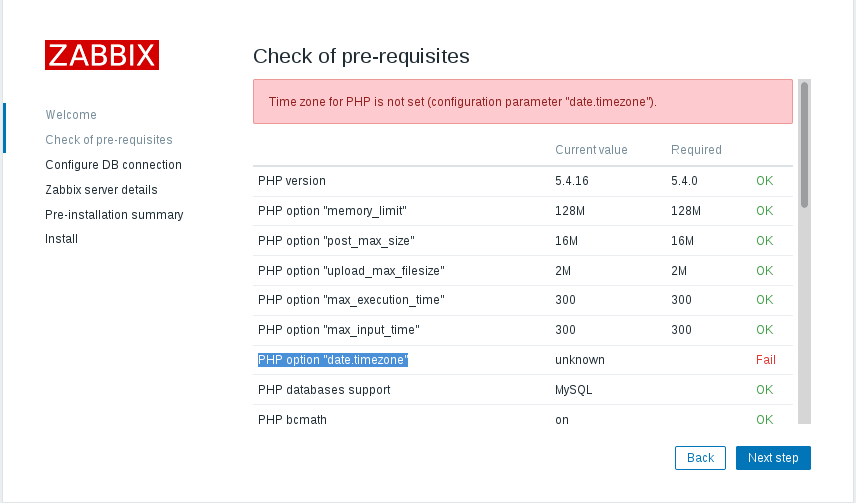
\includegraphics[width=1.0\textwidth]{images/timezone.png}
			\caption{Error date.timezone}
		\end{figure}
	
		Para ellos, vamos a modificar la configuración de php, desde el fichero de configuración "php.ini" de \textbf{apache2}.
		\newline
		\newline
		
\begin{tikzpicture}[node distance=-0.5em]
		\node[
			anchor=north,
			draw=black,
			fill=black,
			inner xsep=0.5cm,
			inner ysep=0.2cm,
			line width=4pt,
			text width=\textwidth - 1cm,
			align=left
		] (box) { {\color{command}\textbf{vi}} {\color{param} /etc/php/7.0/apache2/\textbf{php.ini}}};
		\node[
			fill=black,
			rounded corners
		] at (box.west) {\color{white}$\boldsymbol{>}$};
		\end{tikzpicture}
		\newline
		\newline
		Ahora vamos a buscar la línea que aparece "\textit{date.timezone}" y después del igual vamos a decir la zona horaria entre comillas que queremos, en nuestro caso \textbf{"Europe/Madrid"}.
		\newline
		\newline
		Finalmente, podemos activar, iniciar y reiniciar todos los servicios:
		\newline
		\newline
		
\begin{tikzpicture}[node distance=-0.5em]
		\node[
			anchor=north,
			draw=black,
			fill=black,
			inner xsep=0.5cm,
			inner ysep=0.2cm,
			line width=4pt,
			text width=\textwidth - 1cm,
			align=left
		] (box) { {\color{command}\textbf{systemctl}} {\color{flag} enable} {\color{param} zabbix-server}};
		\node[
		fill=black,
		rounded corners
		] at (box.west) {\color{white}$\boldsymbol{>}$};
		\end{tikzpicture}
		
\begin{tikzpicture}[node distance=-0.5em]
		\node[
		anchor=north,
		draw=black,
		fill=black,
		inner xsep=0.5cm,
		inner ysep=0.2cm,
		line width=4pt,
		text width=\textwidth - 1cm,
		align=left
		] (box) { {\color{command}\textbf{systemctl}} {\color{flag} start} {\color{param} zabbix-server}};
		\node[
		fill=black,
		rounded corners
		] at (box.west) {\color{white}$\boldsymbol{>}$};
		\end{tikzpicture}
		
\begin{tikzpicture}[node distance=-0.5em]
		\node[
		anchor=north,
		draw=black,
		fill=black,
		inner xsep=0.5cm,
		inner ysep=0.2cm,
		line width=4pt,
		text width=\textwidth - 1cm,
		align=left
		] (box) { {\color{command}\textbf{systemctl}} {\color{flag} restart} {\color{param} apache2}};
		\node[
		fill=black,
		rounded corners
		] at (box.west) {\color{white}$\boldsymbol{>}$};
		\end{tikzpicture}
		\newpage
		Finalmente, debemos configurar el firewall para así poder abrir la monitorización web de \textbf{Zabbix}. El puerto que tendremos que habilitar es el \textbf{puerto 80} con el protocolo de control de transmisión, \textit{tcp}.
		\newline
		\newline
		
\begin{tikzpicture}[node distance=-0.5em]
		\node[
			anchor=north,
			draw=black,
			fill=black,
			inner xsep=0.5cm,
			inner ysep=0.2cm,
			line width=4pt,
			text width=\textwidth - 1cm,
			align=left
		] (box) { {\color{command}\textbf{ufw}} {\color{flag} allow} {\color{param} 80/tcp}};
		\node[
		fill=black,
		rounded corners
		] at (box.west) {\color{white}$\boldsymbol{>}$};
		\end{tikzpicture}
		\newline
		\newline
		Ahora podemos acceder a la dirección "\textit{192.168.56.105/zabbix}" y pulsar Next, además, veremos \textbf{todos} los flags {\color{green} correctos}.
		\newline
		En el siguiente paso nos pedirá la contraseña que hemos utilizado para nuestra base de datos y le daremos un nombre a nuestro servidor.
		\newline
		\newline
		% https://www.zabbix.com/forum/zabbix-troubleshooting-and-problems/16020-how-to-reset-the-admin-password-without-gui-access
		Una vez accedida a la interfaz, podremos entrar en ella utilizando el usuario \textit{Admin} y su contraseña \textit{zabbix}. Si por ejemplo quisiéramos cambiar la contraseña o el nombre, podríamos hacerlo directamente desde el gestor \textbf{MySQL} y alterando de la tabla \textbf{users}, la casilla passwd en formato \textbf{md5}[5] del usuario \textbf{Admin}.
		\newline
		\newline
		Vamos ahora a instalar \textit{Zabbix Agent}, es decir, el cliente.
		\newline
		\newline
		
\begin{tikzpicture}[node distance=-0.5em]
		\node[
		anchor=north,
		draw=black,
		fill=black,
		inner xsep=0.5cm,
		inner ysep=0.2cm,
		line width=4pt,
		text width=\textwidth - 1cm,
		align=left
		] (box) { {\color{command}\textbf{apt}} {\color{flag} install -y} {\color{param} zabbix-agent}};
		\node[
		fill=black,
		rounded corners
		] at (box.west) {\color{white}$\boldsymbol{>}$};
		\end{tikzpicture}
		Como la configuración del puerto ya está hecha, podemos finalmente arrancar el servicio.
		\newline
		\newline
		
\begin{tikzpicture}[node distance=-0.5em]
		\node[
		anchor=north,
		draw=black,
		fill=black,
		inner xsep=0.5cm,
		inner ysep=0.2cm,
		line width=4pt,
		text width=\textwidth - 1cm,
		align=left
		] (box) { {\color{command}\textbf{systemctl}} {\color{flag} enable} {\color{param} zabbix-agent}};
		\node[
		fill=black,
		rounded corners
		] at (box.west) {\color{white}$\boldsymbol{>}$};
		\end{tikzpicture}
		\newline
		\newline
		
\begin{tikzpicture}[node distance=-0.5em]
		\node[
		anchor=north,
		draw=black,
		fill=black,
		inner xsep=0.5cm,
		inner ysep=0.2cm,
		line width=4pt,
		text width=\textwidth - 1cm,
		align=left
		] (box) { {\color{command}\textbf{systemctl}} {\color{flag} start} {\color{param} zabbix-agent}};
		\node[
		fill=black,
		rounded corners
		] at (box.west) {\color{white}$\boldsymbol{>}$};
		\end{tikzpicture}
		\newline
		\newline
		Finalmente ya estaría configurado el servidor, \textit{frontend} y el cliente en \textbf{Ubuntu}, más en adelante veremos como utilizar el \textit{frontend} para monitorizar nuestro agente.
		
		\newpage
		\subsubsection{Intalación Zabbix en CentOS}
		Vamos a realizar de forma parecida a Ubuntu la instalación del agente.\newline
		En primer lugar, vamos a descargarnos el repositorio, para ello vamos a necesitar el paquete \textbf{rpm} .
		\newline
		\newline
		
\begin{tikzpicture}[node distance=-0.5em]
		\node[
			anchor=north,
			draw=black,
			fill=black,
			inner xsep=0.5cm,
			inner ysep=0.2cm,
			line width=4pt,
			text width=\textwidth - 1cm,
			align=left
		] (box) { {\color{command}\textbf{rpm}} {\color{flag} -ivh} {\color{param} https://repo.zabbix.com/zabbix/3.4/rhel/7/x86\_64/zabbix-release-3.4-2.el7.noarch.rpm}};
		\node[
			fill=black,
			rounded corners
		] at (box.west) {\color{white}$\boldsymbol{>}$};
		\end{tikzpicture}
		\newline
		\newline
		Una vez descargado, instalamos el agente con \textbf{yum}.
		\newline
		\newline
		
\begin{tikzpicture}[node distance=-0.5em]
		\node[
		anchor=north,
		draw=black,
		fill=black,
		inner xsep=0.5cm,
		inner ysep=0.2cm,
		line width=4pt,
		text width=\textwidth - 1cm,
		align=left
		] (box) { {\color{command}\textbf{yum}} {\color{flag} install -y} {\color{param} zabbix-agent}};
		\node[   
		fill=black,
		rounded corners
		] at (box.west) {\color{white}$\boldsymbol{>}$};
		\end{tikzpicture}
		\newline
		\newline
		A la hora de iniciar el servicio, nos dará un error, ya que se ha superado un límite de recursos (\textbf{zabbix\_agent\_setrlimit}).
		\newline
		\newline
		
\begin{tikzpicture}[node distance=-0.5em]
		\node[
			anchor=north,
			draw=black,
			fill=black,
			inner xsep=0.5cm,
			inner ysep=0.2cm,
			line width=4pt,
			text width=\textwidth - 1cm,
			align=left
		] (box) { {\color{command}\textbf{cat}} {\color{param} /var/log/audit/audit.log} {\color{flag} $\mid$} {\color{command}\textbf{grep}} {\color{param} zabbix\_agentd} {\color{flag} $\mid$} {\color{command}\textbf{grep}} {\color{param} denied} {\color{flag} $\mid$} {\color{command}\textbf{audit2allow}} {\color{flag} -M} {\color{param} zabbix\_agent\_setrlimit}};
		\node[   
		fill=black,
		rounded corners
		] at (box.west) {\color{white}$\boldsymbol{>}$};
		\end{tikzpicture}
		\newline
		\newline
		Ahora vamos a re-construir e instalar la política del módulo que hemos modificado, para ellos: 
		\newline
		\newline
		
\begin{tikzpicture}[node distance=-0.5em]
		\node[
		anchor=north,
		draw=black,
		fill=black,
		inner xsep=0.5cm,
		inner ysep=0.2cm,
		line width=4pt,
		text width=\textwidth - 1cm,
		align=left
		] (box) { {\color{command}\textbf{semodule}} {\color{flag} -i} {\color{param} zabbix\_agent\_setrlimit.pp}};
		\node[   
		fill=black,
		rounded corners
		] at (box.west) {\color{white}$\boldsymbol{>}$};
		\end{tikzpicture}
		\newline
		\newline
		Ahora este error dejará de aparecer una vez iniciemos los servicios, pero antes, vamos a configurar el servidor en el archivo de configuración del agente.
		\newline
		\newline
		
\begin{tikzpicture}[node distance=-0.5em]
		\node[
		anchor=north,
		draw=black,
		fill=black,
		inner xsep=0.5cm,
		inner ysep=0.2cm,
		line width=4pt,
		text width=\textwidth - 1cm,
		align=left
		] (box) { {\color{command}\textbf{vi}} {\color{param} /etc/zabbix/zabbix\_agentd.conf}};
		\node[   
		fill=black,
		rounded corners
		] at (box.west) {\color{white}$\boldsymbol{>}$};
		\end{tikzpicture}
		\newline
		\newline
		Buscaremos las líneas "\textbf{Server}" y "\textbf{ServerActive}" y ahí añadiremos la ip de nuestro servidor, de igual forma, después del igual.
		\newline
		\newline
		Nos que abrir el puerto de escucha para CentOS y Ubuntu y así se puedan comunicar, para Zabbix, \textbf{habilitaremos el puerto 10050}.
		\newline
		Finalmente, habilitaremos e iniciaremos el servicio \textbf{zabbix-agent} mediante \textbf{systemctl}.
		
		\newpage
		
	\subsection{Monitorización de Zabbix}
		
		Para añadir \textbf{CentOS} a monitorizar[6], vamos a acceder al panel de monitorización:
		
		\begin{figure}[h]
			\centering
			
\includegraphics[width=1.0\textwidth]{images/host.png}
			\caption{Pasos para la configuración de un nuevo host}
		\end{figure}
		Vamos a introducir los datos que se nos piden, además crearemos un nuevo grupo, en nuestro caso lo llamaremos "\textbf{ISE}".
		\newline
		\begin{figure}[h]
			\centering
			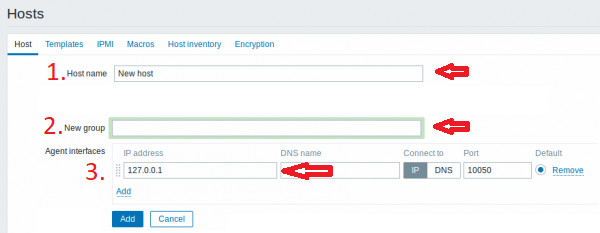
\includegraphics[width=1.0\textwidth]{images/newhost.png}
			\caption{Datos para la configuración de un nuevo host}
		\end{figure}
		\newline
		Una vez introducido estos datos, le damos a \textbf{Add} y nos llevará a una visualización de todos los hosts.
		\newline
		\newline
		Para activar la monitorización de Ubuntu, le daremos click a su estado.
		\newline
		\begin{figure}[h]
			\centering
			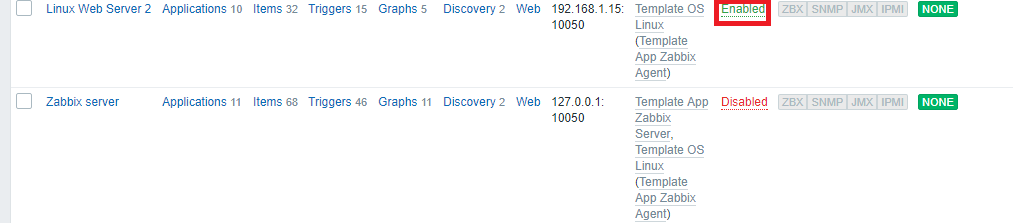
\includegraphics[width=1.0\textwidth]{images/acthost.png}
			\caption{Datos para la configuración de un nuevo host}
		\end{figure}
	\newpage
	\subsection{Gráficas de Zabbix}
		Podemos ver el rendimiento de nuestro grupo de servidores o por separado a través de la pantalla \textbf{Graphs}.
		\newline
		\begin{figure}[h]
			\centering
			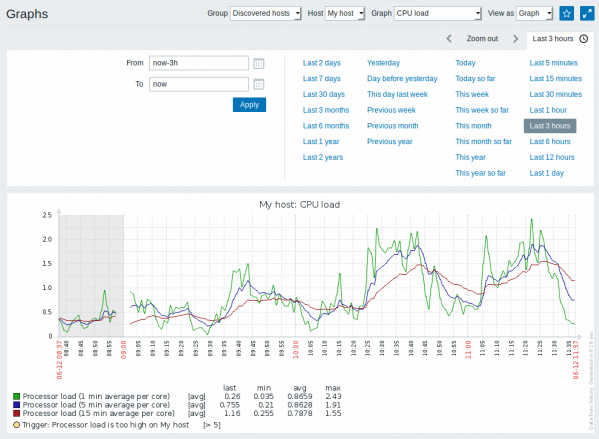
\includegraphics[width=1.0\textwidth]{images/graphs.png}
			\caption{Gráfico de nuestro grupo / único host}
		\end{figure}
	
	
	\newpage
	\section{Referencias Bibliográficas}
	\begin{thebibliography}{9}
		\bibitem{Zabbix}
		¿Qué es Zabbix?
		\url{https://es.wikipedia.org/wiki/Zabbix}
		
		\bibitem{Ubuntu}
		El sistema operativo Ubuntu
		\url{https://es.wikipedia.org/wiki/Ubuntu}
		
		\bibitem{Ubuntu}
		El sistema operativo CentOS
		\url{https://es.wikipedia.org/wiki/CentOS}
		
		\bibitem{Instalacion}
		Instalación de Zabbix Server y Cliente
		\url{https://proyectos.softwarelibre.edu.uy/projects/gestion-de-la-sala-de-telecomunicaciones/wiki/Configuracion_de_Zabbix_Server_y_Zabbix_Client}
		
		\bibitem{Linux Apache MySQL PHP}
		Instalación de Zabbix Server y Cliente
		\url{https://es.wikipedia.org/wiki/LAMP}
		
		
		\bibitem{Frontend Zabbix}
		Monitorizar y Gráficos en Zabbix
		\url{https://tecadmin.net/add-host-zabbix-server-monitor/}
		
		
	\end{thebibliography}
		
\end{document}